%!TEX encoding = UTF-8 Unicode

%!TEX root = ../compendium.tex

\Lab{\LabWeekSIX}

\begin{Goals}
\item Kunna skapa egna klasser.
\item Förstå skillnaden mellan klasser och objekt.
\item Förstå skillnaden mellan muterbara och omuterbara objekt.
\item Förstå hur ett objekt kan innehålla referenser till objekt av andra klasser, och varför detta kan vara användbart.
\item Träna på att fatta beslut om vilka datatyper som bäst passar en viss tillämpning.
\end{Goals}

\begin{Preparations}
\item \DoExercise{\ExeWeekSIX}{06}

\item Studera dokumentationen för klassen \jcode{cslib.window.SimpleWindow} här: \url{http://cs.lth.se/pgk/api/}


\end{Preparations}

\subsection{Bakgrund}

Under den här laborationen ska du skriva en samling av klasser som tillsammans kan användas för att rita i ett fönster. För att ge dig en grund att stå på får du tillgång till den färdigskrivna klassen SimpleWindow. SimpleWindow är en Java-klass som kan skapa ett enkelt ritfönster på skärmen, med metoder för att rita linjer, etc. SimpleWindow håller koll på en ''penna'' som representerar \textit{aktuell ritposition}. Det finns metoder för att flytta pennan och att rita en rak linje från pennans aktuella ritposition till en ny pennposition.

Med hjälp av SimpleWindow ska du skapa en Turtle-klass, som ska fungera likt sköldpaddan i Kojo, vilken du använde i laborationen i avsnitt \ref{section:lab:kojo}. Delar av \href{http://cs.lth.se/pgk/api/}{dokumentationen} för SimpleWindow återspeglas i nedan specifikation.

\vspace{1em}%hack to keep comment with method
\begin{JavaSpec}{class SimpleWindow}
  /** mouse click event type */
	public final static int MOUSE_EVENT = 1;

  /** key pressed event type */
	public final static int KEY_EVENT = 2;

  /** window closed event type */
	public final static int CLOSE_EVENT = 3;

  /** Creates a window and makes it visible. */
	public SimpleWindow(int width, int height, String title);

  /** Returns the width of the window. */
	public int getWidth();

	/** Returns the height of the window. */
	public int getHeight();

	/** Clears the window. */
	public void clear();

	/** Closes the window.*/
	public void close();

	/** Opens the window. */
	public void open(); 

	/** Moves the pen to a new position. */
	public void moveTo(int x, int y) ;

	/** Moves the pen to a new position while drawing a line. */
	public void lineTo(int x, int y);

	/** Writes a string at the current position.* /
	public void writeText(String txt);
	
	/** Draws a bitmap image at the current position.*/
	public void drawImage(Image image);

	/** Returns the pen's x coordinate. */
	public int getX();

	/** Returns the pen's y coordinate. */
	public int getY();

	/** Sets the line width.  */
	public void setLineWidth(int width);

	/** Sets the line color. */
	public void setLineColor(Color col);

	/**Returns the current line width. */
	public int getLineWidth();

	/** Returns the current line color. */
	public Color getLineColor();
	
	/**  Waits for a mouse click. */
	public void waitForMouseClick();

	/** Returns the mouse x coordinate at the last mouse click. */
	public int getMouseX();

	/** Returns the mouse y coordinate at the last mouse click. */
	public int getMouseY();

	/**Adds a sprite to the window. */
	public void addSprite(Sprite sprite);

	/** Wait for a specified time. */
	public static void delay(int ms);


\end{JavaSpec}




\clearpage

\subsection{Obligatoriska uppgifter}

\Task Skapa en klass Point för att beskriva en viss koordinat (x,y) i ett fönster. Klassen ska vara omuterbar - man ska alltså inte kunna ändra på en koordinat efter att den har skapats. Notera att klassens attribut är av typen Double och inte Int, trots att de i någon mån beskriver en diskret pixelposition. Anledningen till detta är att det kan uppstå avrundningsfel vid upprepade förflyttningar. Detta blir särskilt märkbart då varje förflyttning är liten, som t.ex. när en Turtle används för att rita en cirkel.

\ScalaSpecInputListing{Point}{../workspace/w06_turtlegraphics/src/main/scala/turtlegraphics/Point.scala}

\Subtask Implementera klassen Point.

\Task Skapa klassen Turtle:

\ScalaSpecInputListing{Turtle}{../workspace/w06_turtlegraphics/src/main/scala/turtlegraphics/Turtle.scala}

\Subtask Vilka attribut finns i klassen, och vilken synlighetsnivå har de? Vilken/vilka konstruktorer finns? 

\Subtask Är klassen muterbar eller omuterbar? Motivera! Hade man kunnat göra tvärtom?

\Subtask Implementera klassen Turtle enligt specifikationen ovan. När klassen är färdigimplementerad ska den kunna användas för att rita figurer från labbens main-metod i filen Main.scala.

\ScalaSpecInputListing{Main}{../workspace/w06_turtlegraphics/src/main/scala/turtlegraphics/Main.scala}

\Subtask Kör main-metoden ovan för att bekräfta att din implementation fungerar. Bilden ska visa två lika stora rektanglar i samma höjd.

\Subtask Just nu behöver användaren av en Turtle specificera alla detaljer om en Turtles ursprungliga tillstånd som parametervärden för att skapa den. För att underlätta för användaren ska du nu skapa en alternativ konstruktor som kräver färre parametrar. Vilka konstruktorparametrar skulle kunna bytas ut mot rimliga default-värden?

\Subtask Använd din Turtle för att rita en cirkel. För att göra detta kan du t.ex. låta din Turtle gå ett kort steg och svänga någon grad tills den har gjort ett fullt varv.

\Subtask Skapa två stycken Turtles i samma fönsterobjekt som rör sig alternerande. Fungerar allt som tänkt?

\begin{itemize}
\item \textbf{Tips}: SimpleWindow har sitt origo i övre vänstra hörnet (och inte det nedre vänstra hörnet som är vanligt inom matematik).
\end{itemize}

\Task Skapa klassen Rectangle: 

\vspace{1em}%hack to keep comment with method
\ScalaSpecInputListing{Rectangle}{../workspace/w06_turtlegraphics/src/main/scala/turtlegraphics/Rectangle.scala}

\Subtask Vilken synlighetsnivå bör konstruktorparametrarna ges? Motivera.

\Subtask I specifikationen står det att rektangeln roteras runt det övre vänstra hörnet, men finns det andra val av rotationsaxlar? Vilka fördelar/nackdelar finns för olika val?
Välj den implementationen du anser lämpligast.

\Subtask Implementera klassen Rectangle enligt specifikationen ovan.

\Subtask Använd din Rectangle för att skapa en animation som utnyttjar skalning, rotation och förflyttning.
Du kan skapa en animering genom att använda dig av SimpleWindow-objektens clear-metod för att rensa skärmen, samt SimpleWindow-klassens delay-metod.
Notera att delay-metoden inte kan anropas på objektet. Se nedanstående exempel.

\begin{Code}
val w = new SimpleWindow(500,500, "Animation")
while(true){
	w.clear()
	// Draw something here
	SimpleWindow.delay(50)
}
\end{Code}


\clearpage

\subsection{Frivilliga extrauppgifter}


\Task Skapa en klass RectangleSequence. I denna klass skall draw-metoden rita ut ett antal rektanglar där varje rektangel har förflyttat sig, roterats och skalats jämfört med föregående rektangel i sekvensen. Se bilder nedan.


\ScalaSpecInputListing{RectangleSequence}{../workspace/w06_turtlegraphics/src/main/scala/turtlegraphics/RectangleSequence.scala}

\Subtask Implementera RectangleSequence.

\Subtask I SimpleWindow kan man ange en färg via metoden setLineColor som ska användas vid utritning. Nyttja detta för att göra en färggladare visualisering av rektangelsekvensen.

\Subtask RectangleSequence är resultatet av flera lager utav abstraktioner. Vilka abstraktionslager ser du? Skulle man kunna abstrahera ytterligare?

\begin{figure}[H]
\centering
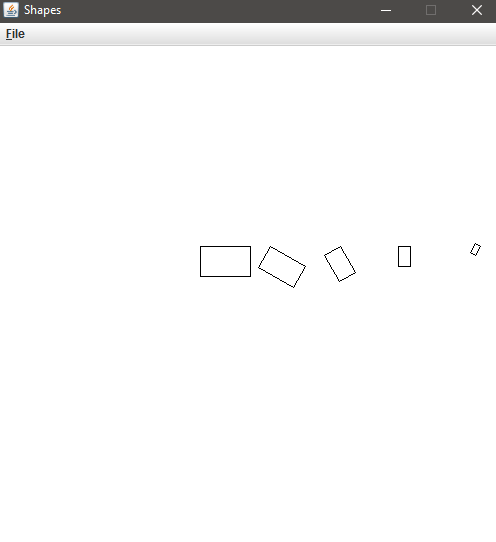
\includegraphics[width=0.7\textwidth, height = 0.3\pdfpageheight, keepaspectratio]{../img/w06-lab/RollingRectangle.png}
\caption {Resultatet av: \newline \texttt{RectangleSequence(\newline \mbox{~~Rectangle(Point(200, 200), 50, 30, 0), 5, 0, 70, -30, 0.67}\\) }}
\label{fig:classes:turtlegraphics:rollingrectangle}
\end{figure}

\begin{figure}[H]
\centering
\begin{Code}
val w = new SimpleWindow(500, 500, "Shapes")
val t = new Turtle(w, new Point(200, 200), 0, false)
val rect = Rectangle(Point(225, 235), 50, 30, 0)
val roll = RectangleSequence(rect, 100, 0, 2, 0, 0.98)
for(i <- 0 to 360 by 20) {
  roll.rotateLeft(i).draw(t)
} 
\end{Code}
\caption {Kod som ritar bilden som visas i figur \ref{fig:classes:turtlegraphics:rectanglesequence} på sidan \pageref{fig:classes:turtlegraphics:rectanglesequence}.}
\label{fig:classes:turtlegraphics:rectanglesequence:code}
\end{figure}


\begin{figure}[H]
\centering
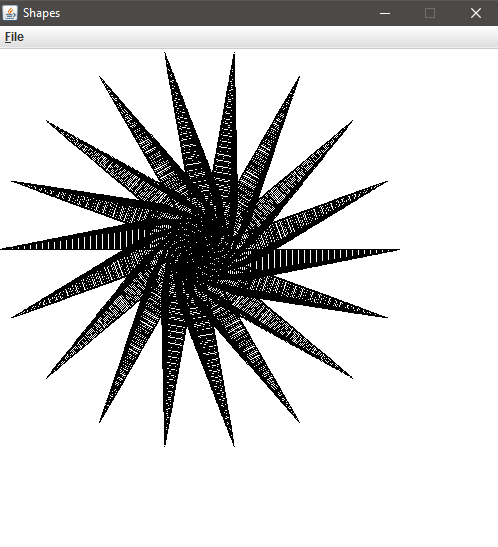
\includegraphics[width=0.7\textwidth, height = 0.3\pdfpageheight,keepaspectratio]{../img/w06-lab/RectangleSequence.png}
\caption {Resultatet av koden i figur \ref{fig:classes:turtlegraphics:rectanglesequence:code}.}
\label{fig:classes:turtlegraphics:rectanglesequence}

\end{figure}


\Task Studera dokumentationen för de SimpleWindow-metoder som erbjuder hantering av händelser \Eng{event} och använd dessa för lösa deluppgifterna nedan.

\Subtask Gör så att en Turtle kan styras med hjälp av tangentbordstryckningar A--S--D--W för vänster--ner--höger--upp och att den ritar ett spår allteftersom den förflyttas. 

\Subtask Gör så att en andra Turtle kan styras med hjälp av tangentbordstryckningar J--K--L--I för vänster--ner--höger--upp och att den också ritar ett spår allteftersom den förflyttas. 

\Subtask Gör så att, när de två sköldpaddorna ovan befinner sig tillräckligt nära varandra, det ritas ut en rektangel med hörn där de två sköldpaddorna finns. (Denna uppgift är lite svårare och kan behöva delas upp i delar.)


\Task Studera dokumentationen för de SimpleWindow-metoder som erbjuder hantering av flyttbara bilder \Eng{sprites}. Gör så att en fin Sprite ritas vid positionen för de styrbara sköldpaddorna i föregående uppgift.

\Task En riktig utmaning, för den som har lust: Implementera spelet ''Masken'' som beskrivs här: \url{https://sv.wikipedia.org/wiki/Snake}.